% Options for packages loaded elsewhere
\PassOptionsToPackage{unicode}{hyperref}
\PassOptionsToPackage{hyphens}{url}
\documentclass[
  10pt,
  a4paper,
]{article}
\usepackage{xcolor}
\usepackage[margin=22mm]{geometry}
\usepackage{amsmath,amssymb}
\setcounter{secnumdepth}{-\maxdimen} % remove section numbering
\usepackage{iftex}
\ifPDFTeX
  \usepackage[T1]{fontenc}
  \usepackage[utf8]{inputenc}
  \usepackage{textcomp} % provide euro and other symbols
\else % if luatex or xetex
  \usepackage{unicode-math} % this also loads fontspec
  \defaultfontfeatures{Scale=MatchLowercase}
  \defaultfontfeatures[\rmfamily]{Ligatures=TeX,Scale=1}
\fi
\usepackage{lmodern}
\ifPDFTeX\else
  % xetex/luatex font selection
\fi
% Use upquote if available, for straight quotes in verbatim environments
\IfFileExists{upquote.sty}{\usepackage{upquote}}{}
\IfFileExists{microtype.sty}{% use microtype if available
  \usepackage[]{microtype}
  \UseMicrotypeSet[protrusion]{basicmath} % disable protrusion for tt fonts
}{}
\makeatletter
\@ifundefined{KOMAClassName}{% if non-KOMA class
  \IfFileExists{parskip.sty}{%
    \usepackage{parskip}
  }{% else
    \setlength{\parindent}{0pt}
    \setlength{\parskip}{6pt plus 2pt minus 1pt}}
}{% if KOMA class
  \KOMAoptions{parskip=half}}
\makeatother
\usepackage{graphicx}
\makeatletter
\newsavebox\pandoc@box
\newcommand*\pandocbounded[1]{% scales image to fit in text height/width
  \sbox\pandoc@box{#1}%
  \Gscale@div\@tempa{\textheight}{\dimexpr\ht\pandoc@box+\dp\pandoc@box\relax}%
  \Gscale@div\@tempb{\linewidth}{\wd\pandoc@box}%
  \ifdim\@tempb\p@<\@tempa\p@\let\@tempa\@tempb\fi% select the smaller of both
  \ifdim\@tempa\p@<\p@\scalebox{\@tempa}{\usebox\pandoc@box}%
  \else\usebox{\pandoc@box}%
  \fi%
}
% Set default figure placement to htbp
\def\fps@figure{htbp}
\makeatother
\setlength{\emergencystretch}{3em} % prevent overfull lines
\providecommand{\tightlist}{%
  \setlength{\itemsep}{0pt}\setlength{\parskip}{0pt}}
\usepackage{mathrsfs}
\usepackage{mathtools}
\usepackage{xurl}
\emergencystretch=3em
\setcounter{tocdepth}{1}
\newcommand{\Beta}{\mathrm{B}}
\DeclareUnicodeCharacter{00B2}{\ensuremath{^2}}
\DeclareUnicodeCharacter{00B1}{\ensuremath{\pm}}
\DeclareUnicodeCharacter{00D7}{\ensuremath{\times}}
\DeclareUnicodeCharacter{2192}{\ensuremath{\to}}
\DeclareUnicodeCharacter{21A6}{\ensuremath{\mapsto}}
\DeclareUnicodeCharacter{2208}{\ensuremath{\in}}
\DeclareUnicodeCharacter{2209}{\ensuremath{\notin}}
\DeclareUnicodeCharacter{2212}{\ensuremath{-}}
\DeclareUnicodeCharacter{2227}{\ensuremath{\wedge}}
\DeclareUnicodeCharacter{2228}{\ensuremath{\vee}}
\DeclareUnicodeCharacter{2260}{\ensuremath{\ne}}
\DeclareUnicodeCharacter{2264}{\ensuremath{\le}}
\DeclareUnicodeCharacter{2265}{\ensuremath{\ge}}
\DeclareUnicodeCharacter{2297}{\ensuremath{\otimes}}
\usepackage{bookmark}
\IfFileExists{xurl.sty}{\usepackage{xurl}}{} % add URL line breaks if available
\urlstyle{same}
\hypersetup{
  hidelinks,
  pdfcreator={LaTeX via pandoc}}

\author{}
\date{}

\begin{document}

{
\setcounter{tocdepth}{3}
\tableofcontents
}
\section{Infinitesimal vanishing, retained currents, and support-valued
positivity}\label{infinitesimal-vanishing-retained-currents-and-support-valued-positivity}

22 September 2026. This note computes the several different vanishing
statements at the observed collision, the complete signs that survive,
and the exact class of corrections capable of changing them. The
calculations retain the original observation, metric, Hermitian summand,
amplitude multiplier, and full support algebra. No off-line zero of the
Riemann zeta function is asserted to exist.

The incoming public programme proofs are
\href{https://github.com/KokunoYumeto/zeta-function-research-reader/blob/c9df443d9e1df000dfbb083943f97197e746eb08/workbenches/splitzero-tandem/branches/identity-absorber-square/OBSERVED_COLLISION.md}{\emph{The
observed infinitesimal collision and the full arithmetic operator},
OC1--OC17};
\href{https://github.com/KokunoYumeto/zeta-function-research-reader/blob/c9df443d9e1df000dfbb083943f97197e746eb08/workbenches/splitzero-tandem/branches/identity-absorber-square/OBSERVED_SUPPORT_PROPAGATION.md}{\emph{Observed
support at the shifted nilpotent collision}, OSP1--OSP42}; and
\href{https://github.com/KokunoYumeto/zeta-function-research-reader/blob/c9df443d9e1df000dfbb083943f97197e746eb08/workbenches/splitzero-tandem/branches/identity-absorber-square/OBSERVED_COTANGENT_FROBENIUS.md}{\emph{Cotangent
and Frobenius calculations for the observed collision}, OCF1--OCF23 and
OIF1--OIF36}. The additional complete local dependencies are
\href{https://github.com/KokunoYumeto/zeta-function-research-reader/blob/173dbc6ed5a03235dbe7654f928f3692107db39b/workbenches/splitzero-tandem/branches/tau-zero-prime-positivity/FULL_SUPPORT_RECONSTRUCTION_DERIVATION.md}{full-support
reconstruction proof}, FSR1--FSR36;
\href{https://github.com/KokunoYumeto/zeta-function-research-reader/blob/173dbc6ed5a03235dbe7654f928f3692107db39b/workbenches/splitzero-tandem/branches/tau-zero-prime-positivity/WEIL_PACKET_DERIVATION.md}{finite
Weil packet proof}, WP1--WP57; and
\href{https://github.com/KokunoYumeto/zeta-function-research-reader/blob/173dbc6ed5a03235dbe7654f928f3692107db39b/workbenches/splitzero-tandem/branches/tau-zero-prime-positivity/WEIL_PACKET_ANALYTIC_DERIVATION.md}{analytic
Weil packet proof}, WA1--WA30. Their complete sources accompany this
derivation; no public link is asserted for an unpublished dependency.
The cited proofs retain their original human citations. This is a
further finite derivation and an application of the already proved
analytic identity WA24, not a replacement for its analytic proof.

\subsection{1. Original operators and the
collision}\label{original-operators-and-the-collision}

Keep the original source data and metric from OC1--OC3: \[
M=C+R,\quad C=C^\dagger,\quad R=\epsilon fe^\dagger,
\quad e^\dagger e=f^\dagger f=1,\quad e^\dagger f=0,\quad\epsilon>0,
\] \[
J=G_N^{-1}\Lambda^*Q_B^{1/2},\quad
Q_B=(\Lambda G_N^{-1}\Lambda^*)^{-1},\quad J^\dagger J=I_B,
\quad C_B=J^\dagger CJ=C_B^*.
\tag{ISP1}
\] Here the original arithmetic quotient, cutoff, and observation remain
those of OC1: \(q=(k+1)^2\), \(k\ge17\), \(k\equiv1\pmod4\),
\(q-1\le N\le2q\), and the original surjection \(\Lambda:E\to B\). The
star is the adjoint in the Euclidean coordinates supplied by the
isometry \(J\); it does not change the original metric.

Write \[
u=J^\dagger e,\quad v=J^\dagger f,\quad
a=u^*u,\quad r=u^*v,\quad d=v^*v,\quad
\Delta=ad-|r|^2>0.
\] The measured area statement in OC3 supplies this strict inequality.
Define \[
g=u/\sqrt a,\qquad
h=\frac{v-(r/a)u}{\sqrt{\Delta/a}},\qquad
b=\epsilon\sqrt\Delta>0,\qquad P=gg^*+hh^*.
\tag{ISP2}
\] The numerator defining \(h\) has inner product zero with \(u\),
because \(u^*v-(r/a)u^*u=0\). Its squared norm is
\(d-|r|^2/a=\Delta/a\). Thus \(g,h\) are an orthonormal pair and \(P\)
is their orthogonal projector.

The exact observed family is \[
F_B(s)=(\epsilon v+su)u^*,\qquad
M_B(s)=C_B+F_B(s),\qquad
\lambda(s)=as+\epsilon r.
\tag{ISP3}
\] Direct multiplication gives \(F_B(s)^2=\lambda(s)F_B(s)\). On the
original orthogonal plane \(S=\operatorname{im}P\), and on its
orthogonal complement \(H\), respectively, it is \[
F_B(s)|_S=\begin{pmatrix}\lambda(s)&0\\b&0\end{pmatrix},
\qquad F_B(s)|_H=0.
\tag{ISP4}
\] At the collision parameter \[
s_*=-\epsilon r/a,
\quad N=F_B(s_*)=\epsilon\bigl(v-(r/a)u\bigr)u^*=bhg^*,
\quad N^2=0,\quad Ng=bh\ne0.
\tag{ISP5}
\] The map \(\mathbb C[\eta]/(\eta^2)\to\operatorname{End}(B)\),
\(1\mapsto I_B\), \(\eta\mapsto N\), is injective. Indeed a relation
\(cI_B+\ell N=0\) applied to \(h\) gives \(c=0\), and then applied to
\(g\) gives \(\ell b=0\), hence \(\ell=0\). Its image is exactly the
generated algebra. The supported version sends its unit to \(P\) and has
the same proof on \(S\).

\subsection{2. Exactly what vanishes}\label{exactly-what-vanishes}

For the isolated nilpotent operator, for every scalar \(t\), \[
\operatorname{tr}(N^j)=0\quad(j\ge1),\qquad
\det(I_B-tN)=1,\qquad
(I_B-tN)^{-1}=I_B+tN.
\tag{ISP6}
\] In the basis \(g,h\), \(N\) is strictly triangular, and is zero on
\(H\). This proves the trace and determinant assertions; multiplication
proves the inverse. A marked matrix element retains the exact term \[
x^*((I_B-tN)^{-1}-I_B)y
=tb(x^*h)(g^*y).
\tag{ISP7}
\] For \(x=h,y=g\), this term is \(tb\), which is nonzero when
\(t\ne0\). Vanishing of the isolated trace series therefore has an
explicit kernel and a nonzero receiver.

The family algebra itself is \[
\mathcal A=\mathbb C[t,z]/(z(z-at)),\qquad t=s-s_*.
\] The invertible change \(\xi=z-at/2\), with inverse \(z=\xi+at/2\),
gives \[
z(z-at)=\xi^2-a^2t^2/4.
\tag{ISP8}
\] Over \(\mathbb C[t]/(t^2)\), this is an isomorphism with the constant
dual-number family, and it reduces to the identity on the fibre \(t=0\).
Thus its first-order deformation class vanishes. Over
\(\mathbb C[t]/(t^3)\), the trace discriminant in the basis \(1,z\)
equals \(a^2t^2\ne0\); the constant dual-number family's trace
discriminant is zero. To compute it, multiplication by \(z\) has trace
\(at\), and multiplication by \(z^2=at z\) has trace \(a^2t^2\). The
trace matrix is therefore
\(\left(\begin{smallmatrix}2&at\\at&a^2t^2\end{smallmatrix}\right)\),
with determinant \(a^2t^2\). An invertible basis change multiplies its
determinant by a unit square. Hence it cannot turn this nonzero
discriminant into zero. The first nontrivial order is exactly two.

The original operator representation and its metric retain additional
information. Work now over \(\mathbb C[t]/(t^2)\), and put \[
K=\frac{a}{2b}gh^*,\qquad T=I_B+tK,\qquad T^{-1}=I_B-tK.
\] Since \([K,N]=(a/2)(gg^*-hh^*)\), direct multiplication proves \[
F_B(s_*+t)=TNT^{-1}+\frac{at}{2}P,
\] \[
T^{-1}M_B(s_*+t)T
=C_B+N+t\left([C_B,K]+\frac a2P\right).
\tag{ISP9}
\] Here \(C_B\) remains the original operator on all of \(B\); it need
not preserve \(S\). These formulas follow by expanding products and
using \(t^2=0\). If the formal parameter is given the real involution
\(t^*=t\), then \[
T^*T=I_B+t(K+K^*).
\tag{ISP10}
\] The coefficient \(K+K^*\) is nonzero, because \((K+K^*)h=(a/(2b))g\).
Thus this coordinate trivialization is not unitary for the original
metric. Equations ISP9--ISP10 retain the exact operator and metric
changes attached to the vanishing deformation class.

There is also a choice-dependent Frobenius vanishing. Over a torsionfree
integral collision ring \(D_p=K_p[\eta]/\eta^2\) with the coefficient
Frobenius specified in OIF33, every lift is \[
\Phi_c(\eta)=pc\eta,\qquad c\in K_p.
\tag{ISP11}
\] To verify this, write an image as \(A+B\eta\). Its square is zero, so
the coefficient domain forces \(A=0\). Its reduction must equal
\(\eta^p=0\), forcing \(B\in pK_p\); the converse is immediate. The
corrected lift has \(c=0\), so kills \(\eta\), whereas the earlier
multiplicative lift has \(c=1\) and sends it to \(p\eta\ne0\). The same
underlying nilpotent algebra therefore does not determine this Frobenius
vanishing without the specified lift.

\subsection{3. The full arithmetic determinant does not vanish
infinitesimally}\label{the-full-arithmetic-determinant-does-not-vanish-infinitesimally}

Keep \(C_B\) in the characteristic polynomial, and let \(n=\dim B\).
Rank-one determinant expansion gives \[
\det(\zeta I_B-C_B-N)
=\det(\zeta I_B-C_B)
-b\,g^*\operatorname{adj}(\zeta I_B-C_B)h.
\tag{ISP12}
\] For a proof, expand the determinant column by column. Every term
containing at least two columns from \(bhg^*\) vanishes because those
columns are proportional to \(h\). The terms containing exactly one such
column sum to the displayed adjugate contraction, with the minus sign
from the subtracted perturbation. This proof is a polynomial identity
and does not require an inverse.

In particular, the isolated identity \(\det(I-tN)=1\) does not remove
the second term of ISP12. On the plane, the concrete Hermitian choice
\(C_B|_S=\left(\begin{smallmatrix}0&c\\c&0\end{smallmatrix}\right)\),
\(c\in\mathbb R\setminus\{0\}\), gives \[
\det(\zeta I_S-C_B|_S-N|_S)=\zeta^2-c(c+b),
\qquad \det(\zeta I_S-C_B|_S)=\zeta^2-c^2.
\tag{ISP13}
\] This example disproves an inference from nilpotence alone; it is not
substituted for the native \(C_B\).

For the actual family, define \[
p_*(\zeta)=\det(\zeta I_B-M_B(s_*)),\qquad
q_*(\zeta)=u^*\operatorname{adj}(\zeta I_B-M_B(s_*))u.
\] The same polynomial expansion proves, exactly for every \(t\), \[
p_{s_*+t}(\zeta)=p_*(\zeta)-tq_*(\zeta).
\tag{ISP14}
\] Moreover \(q_*\) has degree \(n-1\) and leading coefficient
\(u^*u=a>0\): the adjugate of \(\zeta I_B-M_B(s_*)\) has leading
coefficient \(\zeta^{n-1}I_B\). Consequently the full characteristic
polynomial has a nonzero first derivative in the original parameter,
even though the abstract algebra deformation class in ISP8 vanishes.
Equivalently,
\(\operatorname{tr}M_B(s_*+t)=\operatorname{tr}M_B(s_*)+at\). These
statements concern the actual original family.

\subsection{4. The signed current survives with both
signs}\label{the-signed-current-survives-with-both-signs}

Use exactly the programme convention \[
W_B(s)=i(M_B(s)-M_B(s)^*).
\] The retained Hermitian term cancels in this particular difference
because \(C_B=C_B^*\). It remains in ISP12--ISP14. Direct conjugate
transposition of ISP4 gives \[
W_B(s)|_S=
\begin{pmatrix}-2\operatorname{Im}\lambda(s)&-ib\\ib&0\end{pmatrix},
\qquad W_B(s)|_H=0.
\tag{ISP15}
\] At the infinitesimal collision, \[
W_*:=W_B(s_*)=i(N-N^*),\qquad
W_*^2=b^2P,
\] \[
W_*\frac{g+ih}{\sqrt2}=b\frac{g+ih}{\sqrt2},\qquad
W_*\frac{g-ih}{\sqrt2}=-b\frac{g-ih}{\sqrt2}.
\tag{ISP16}
\] These follow by multiplying the two-by-two matrix, or by using
\(Ng=bh,Nh=0,N^*h=bg,N^*g=0\). Its inertia on \(B\) is \((1,1,n-2)\).
For \(y=c_g g+c_hh+y_H\), \[
y^*W_*y=2b\operatorname{Im}(\overline{c_g}c_h).
\tag{ISP17}
\] Thus the two unit eigenvectors in ISP16 have values \(+b\) and
\(-b\), not zero.

The current correction from the original parameter \(s=0\) is exactly \[
W_*-W_B(0)=2\epsilon\operatorname{Im}(r)gg^*.
\tag{ISP18}
\] For every complex parameter \(s\), the determinant of its active
matrix in ISP15 is \(-b^2<0\). Consequently that rank-one displacement
cannot make the current positive semidefinite. Along the real
displacement \(s=s_*+t\), \(t\in\mathbb R\), the full current is exactly
constant, \(W_B(s_*+t)=W_*\), because \(\lambda(s_*+t)=at\) is real.

\subsection{5. All Hermitian corrections on the current
plane}\label{all-hermitian-corrections-on-the-current-plane}

Write an arbitrary Hermitian correction on \(S\) as \[
D=\begin{pmatrix}\alpha&c\\\overline c&\delta\end{pmatrix},
\qquad\alpha,\delta\in\mathbb R,\quad c\in\mathbb C.
\] Then the complete set of corrections giving a nonnegative form is \[
\boxed{W_*+D\succeq0
\quad\Longleftrightarrow\quad
\alpha\ge0,\ \delta\ge0,\ \alpha\delta\ge|c-ib|^2.}
\tag{ISP19}
\] For necessity evaluate on \(g,h\), obtaining the diagonal
inequalities, and use the nonnegative determinant. For sufficiency, when
\(\alpha>0\), complete the square: \[
\alpha\left|x+\frac{c-ib}{\alpha}y\right|^2
+\left(\delta-\frac{|c-ib|^2}{\alpha}\right)|y|^2\ge0.
\] When \(\alpha=0\), the determinant inequality forces \(c-ib=0\), and
the form is \(\delta|y|^2\). This proves every boundary case as well as
the positive-definite case.

In particular, an orthogonal-support correction \(tP\),
\(t\in\mathbb R\), gives positivity exactly for \(t\ge b\). A correction
supported only on \(gg^*\), or only on \(hh^*\), never suffices. The
equality \(e^2=e\) by itself supplies no scalar coefficient \(t\); ISP19
states the exact correction needed by the operator it would act on.

The analogous complete classification for a larger support space is as
follows. Let \(X,Z\) be finite-dimensional Hermitian spaces and let \[
\mathcal Q=\begin{pmatrix}H&A\\A^*&D\end{pmatrix}
\quad\text{on }X\oplus Z,
\qquad H=H^*,\quad D=D^*.
\] Let \(D^+\) be the operator equal to the reciprocal of each nonzero
eigenvalue of \(D\) and zero on its kernel. Then \[
\boxed{\mathcal Q\succeq0\quad\Longleftrightarrow\quad
D\succeq0,\quad A(\ker D)=0,\quad H-AD^+A^*\succeq0.}
\tag{ISP20}
\] To prove necessity, first restrict to \(Z\). For \(z_0\in\ker D\),
the value on \((x,tz_0)\) is \(x^*Hx+2\operatorname{Re}(t x^*Az_0)\).
Its nonnegativity for every complex \(t\) forces \(Az_0=0\). Thus
\(A^*x\) belongs to \((\ker D)^\perp=\operatorname{im}D\). For all
\(x,z\), exact multiplication now gives \[
\langle(x,z),\mathcal Q(x,z)\rangle
=x^*(H-AD^+A^*)x
+(z+D^+A^*x)^*D(z+D^+A^*x).
\tag{ISP21}
\] Set \(z=-D^+A^*x\) for the last necessary inequality. Conversely
ISP21 proves positivity from the three displayed conditions. This proof
constructs the minimizing support coordinate and includes singular
\(D\).

For a fixed Hermitian correction \(R\) to the old block, replace \(H\)
in ISP20 by \(H+R\); the result classifies every such corrected
extension. Adding independent support coordinates and mixed blocks while
leaving \(H\) unchanged cannot remove an old negative value: it is still
the value on \((x,0)\). Indeed minimizing over the added positive
coordinates subtracts \(AD^+A^*\), exactly as ISP21 records.

\subsection{6. Full support and every positive scalar
trace}\label{full-support-and-every-positive-scalar-trace}

Retain the finite bounded distributive lattice \(L\), the actual
semiring \(G_L(R)\), and its supported zero \(e_L\), with \((e_L)=Z_L\)
prime when \(R\) is a domain. This is prior programme mathematics, not a
new result here. The contracted multiplicative algebra is the proved
product \[
\Gamma_L=\mathbb C[(G_L(R),\times)]/([\tau_L])
\cong C_L\times D_R,
\quad C_L=\mathbb C[(L,\wedge)]/([0_L]).
\tag{ISP22}
\] In this algebra \([e_L]\) is the identity of the \(C_L\) factor. It
is a multiplicative idempotent, not the square-zero operator \(N\) of
ISP5. The latter comes from the separate, explicitly specified
deformation/observation receiver. The exact role of the former in the
following coefficient extension is multiplication by the support
identity.

FSR11--FSR14 give \[
C_L=\bigoplus_{a\in L\setminus\{0\}}\mathbb CE_a,
\quad E_aE_b=\delta_{ab}E_a,\quad E_a^*=E_a,
\quad\sum_aE_a=1_{C_L}.
\tag{ISP23}
\] For completeness, the characters are
\(\eta_a([\lambda])=1_{a\le\lambda}\); their incidence matrix is
triangular with diagonal one, hence invertible. Its inverse gives
\(E_a=\sum_{\lambda\le a}\mu(\lambda,a)[\lambda]\). Applying every
character proves the stated multiplication and unit identities.

Every positive complex-linear scalar functional on \(C_L\) is uniquely
\[
\ell\Bigl(\sum_ac_aE_a\Bigr)=\sum_at_ac_a,
\qquad t_a\ge0.
\tag{ISP24}
\] Indeed \(E_a=E_a^*E_a\) forces \(\ell(E_a)\ge0\); conversely the
displayed coefficients give \(\ell(v^*v)=\sum_at_a|v_a|^2\ge0\). It is
faithful on positive elements precisely when every \(t_a>0\).

Extend the actual current coefficientwise to \(B_L=C_L\otimes B\),
retaining \(1\otimes C_B\) in its full arithmetic operator. Its
support-valued form is \[
\mathcal W_L(x,y)=\sum_aE_a x_a^*W_*y_a,
\qquad x=\sum_aE_a\otimes x_a.
\tag{ISP25}
\] For every \(a\) with \(t_a>0\), the exact vector \[
x_a^-=E_a\otimes(g-ih)/\sqrt2
\quad\text{has}\quad
\mathcal W_L(x_a^-,x_a^-)=-bE_a,
\qquad\ell\mathcal W_L(x_a^-,x_a^-)=-bt_a<0.
\tag{ISP26}
\] Thus every nonzero positive functional retains a negative direction
for this form. If exactly \(r\) of the weights are positive and
\(d_L=|L|-1\), its scalar inertia is \[
(r,r,(n-2)r+n(d_L-r)).
\tag{ISP27}
\] This follows by using the two eigenvectors in ISP16 and a basis of
\(H\) in every sector; the sectors of weight zero contribute their
entire \(n\)-dimensional space to the radical.

The same proof applied to the full finite Weil pairing FSR28, whose
scalar inertia is \((2,2,4m-4)\), gives \[
\operatorname{inertia}(\ell\mathbb B_L)
=(2r,2r,(4m-4)r+4m(d_L-r)).
\tag{ISP28}
\] In particular, the regular trace has all weights one. Boolean branch
traces select only join-irreducible sectors and put zero weights on the
remaining mixed sectors; zero observation there does not prove zero full
form. For \(L=\mathbb B^2\), the mixed projector \(w=[1]-[a]-[b]\) obeys
\(w^2=w\ne0\), both branch traces kill it, and FSR34--FSR35 give the
exact value \(-2m w\) on the specified mixed negative packet.

\subsection{7. Exact maps from the collision current to a quartet
packet}\label{exact-maps-from-the-collision-current-to-a-quartet-packet}

This section constructs a finite comparison without identifying it with
the native period observation. Let \(\rho=1/2+\delta+i\gamma\),
\(0<\delta<1/2\), \(\gamma>2\), and use the four distinct points \[
(\alpha_1,\alpha_2,\alpha_3,\alpha_4)
=(\rho,1-\overline\rho,\overline\rho,1-\rho).
\] For \(m\ge1\), let \(d(s)=\prod_i(s-\alpha_i)\), \(h(s)=d(s)^m\),
\(E_h=\mathbb C[s]/(h)\), and let \(e_i\) be the full primary
idempotents. Let \(U=M_{j_h(v)}\) be the original amplitude unit, with
its full Taylor coefficients and nonzero values \(v(\alpha_i)\). Let
\(a_h=\operatorname{ev}U:E_h\to\mathbb C^4\). The finite pairing is \[
B_h(x,y)=m\bigl(\overline{(a_hx)_2}(a_hy)_1+
\overline{(a_hx)_1}(a_hy)_2+
\overline{(a_hx)_4}(a_hy)_3+
\overline{(a_hx)_3}(a_hy)_4\bigr).
\tag{ISP29}
\] These algebraic data can be defined for arbitrary such points and an
arbitrary specified unit; they do not assert a zeta zero.

Define the typed injective linear map \[
\mathcal I:S\longrightarrow E_h,
\quad c_gg+c_hh\longmapsto
\sqrt{b/m}\,U^{-1}(c_ge_1-ic_he_2).
\tag{ISP30}
\] Applying \(a_h\) gives \(\sqrt{b/m}(c_g,-ic_h,0,0)\), so injectivity
follows. Substitution in ISP29 gives the exact isometry \[
B_h(\mathcal I x,\mathcal I y)=x^*W_*y\qquad(x,y\in S).
\tag{ISP31}
\] Explicitly the right side is
\(-ib\overline{x_g}y_h+ib\overline{x_h}y_g\), and the left side has the
same two coefficients. This is an isometry of Hermitian forms, whose
signs are indefinite; it is not asserted to preserve the original
positive norm.

There is also a nilpotent operator on the complete packet, including all
its jets: \[
\mathcal N_h(x)=-ib\,(a_hx)_1 U^{-1}e_2.
\tag{ISP32}
\] Since \((a_hU^{-1}e_2)_1=0\), it has square zero. It is nonzero on
\(U^{-1}e_1\), and direct substitution proves \[
\mathcal N_h\mathcal I=\mathcal I N|_S.
\tag{ISP33}
\] This comparison preserves the constant \(b\), its complex phase, and
the original \(U\). It sends the radical \(J_h=(d)/(d^m)\) to zero by
the formula for \(a_h\); every radical jet remains in the domain and in
\(U\). Extending ISP30--ISP33 by \(C_L\otimes-\) gives the identical
maps in every support sector. The construction is explicit and depends
on the chosen quartet; equality with the original period receiver has
not been asserted or assumed.

\subsection{8. Interpolation removes endpoint terms without changing any
packet
jet}\label{interpolation-removes-endpoint-terms-without-changing-any-packet-jet}

Since none of the four points is \(0\) or \(1\), \(h(0)h(1)\ne0\). For a
polynomial \(q\), set \[
\boxed{\mathcal R_hq(s)=q(s)-h(s)
\left((1-s)\frac{q(0)}{h(0)}+s\frac{q(1)}{h(1)}\right).}
\tag{ISP34}
\] This is a linear polynomial map. Substitution at the two endpoints
gives \[
\mathcal R_hq(0)=\mathcal R_hq(1)=0,
\qquad\mathcal R_hq\equiv q\pmod h.
\tag{ISP35}
\] The latter congruence preserves the derivatives of every order
\(0,\ldots,m-1\) at every \(\alpha_i\), because \(h\) has order \(m\)
there. Conversely divisibility by \(h\) is exactly the kernel of the
complete quartet jet map, by successive division by the four distinct
linear factors. Therefore every original packet class, including every
nilpotent jet and the entire action of \(U\), is retained by this map.

Let \(s_h:E_h\to\mathbb C[s]\) select the unique representative of
degree below \(4m\), as supplied by monic polynomial division. The
composite \[
\widetilde s_h=\mathcal R_hs_h:
E_h\longrightarrow s(s-1)\mathbb C[s]
\tag{ISP36}
\] is a linear section of polynomial reduction modulo \(h\), with degree
at most \(4m+1\). Its image has dimension \(4m\), and every class has
exactly the stated lift. In particular this endpoint condition does not
constrain any quartet jet.

The same statement holds for arbitrary specified finite endpoint orders.
For \(K\ge1\), put \(b_K(s)=s^K(s-1)^K\). It is a unit in \(E_h\),
because each \(b_K(\alpha_i)\ne0\). An explicit inverse is obtained by
the finite Taylor reciprocal in each factor \(\mathbb C[t_i]/(t_i^m)\),
followed by the primary idempotent inverse of the jet map. Consequently
\[
\widetilde s_{h,K}(x)=b_K\,s_h\bigl([b_K]^{-1}x\bigr)
\tag{ISP37}
\] is a linear section of reduction modulo \(h\) whose values vanish to
order at least \(K\) at both \(0\) and \(1\). Multiplication followed by
reduction proves the section identity exactly. This constructs the
connecting map for every finite endpoint jet constraint.

\subsection{9. Consequence for the explicit formula and zero-prime
corrections}\label{consequence-for-the-explicit-formula-and-zero-prime-corrections}

The following application concerns the programme's counterfactual zeta
packet used in WP1--WP4 and WA1--WA2: its four specified points have
exact zero order \(m\) for \(g=2\xi\), so \(v=g/h\) is entire and has
nonzero values there. This is the established test of an off-line
packet; it is not an existence claim.

For two polynomials \(q_1,q_2\), use exactly \[
q^\#(s)=\overline{q(1-\overline s)},\qquad
A_{q_1,q_2}(s)=q_1^\#(s)q_2(s)v(s)^2.
\tag{ISP38}
\] Let \(\widetilde q_i=\mathcal R_hq_i\). Equations ISP35 and WP21
prove that the original full primary amplitude jets of
\(\widetilde q_iv\) and \(q_iv\) agree. Furthermore \[
A_{\widetilde q_1,\widetilde q_2}(0)
=A_{\widetilde q_1,\widetilde q_2}(1)=0.
\tag{ISP39}
\] Indeed the factor \(\widetilde q_2\) vanishes at both endpoints. This
conclusion also follows by evaluating the reflected first factor; no
positivity inference is used.

Take the full-jet negative class \[
x_-=U^{-1}(e_1-e_2),\qquad
\widetilde q_- =\widetilde s_h(x_-).
\tag{ISP40}
\] Its four amplitude values are exactly \((1,-1,0,0)\), hence \[
B_h([\widetilde q_-],[\widetilde q_-])=-2m.
\tag{ISP41}
\] Its Fourier-coordinate polynomial is
\(\widetilde P_-(z)=\widetilde q_-(1/2+iz)\); define
\(F_-(z)=\widetilde P_-(z)v(1/2+iz)\), \[
K_-(t)=|F_-(t)|^2,\qquad
k_-(u)=\frac1{2\pi}\int_{\mathbb R}K_-(t)e^{itu}\,dt.
\] WA9--WA16 apply to every polynomial, so the increased degree in ISP36
changes their constants but not the proved admissibility, exponential
strip decay, or absolute convergence. Substitution into the full
analytic identity WA24, using ISP39, gives \[
\boxed{-2m=
\frac1{2\pi}\int_{\mathbb R}|F_-(t)|^2
\left(\operatorname{Re}\psi(\tfrac14+\tfrac{it}{2})-\log\pi\right)dt
-\sum_{n\ge2}\frac{\Lambda_{\rm ar}(n)}{\sqrt n}
\bigl(k_-(\log n)+k_-(-\log n)\bigr).}
\tag{ISP42}
\] This is the exact endpoint-free arithmetic expression for that
packet, with every sign and transform convention retained. It does not
prove that this packet exists for zeta, and does not prove nonnegativity
of the arithmetic expression.

More generally let \(\mathcal E(q)\) be the vector of any fixed finite
list of derivatives at \(0,1\), and let \(D=D^*\) be any matrix on that
vector space. Every correction \[
\mathcal D(q_1,q_2)=\mathcal E(q_1)^*D\mathcal E(q_2)
\tag{ISP43}
\] vanishes on the image of ISP37 for sufficiently large \(K\). Yet that
image surjects onto every packet jet and contains the negative class
ISP40. The same conclusion holds if \(\mathcal E\) takes the endpoint
jets of \(qv\): multiplication by the entire function \(v\) preserves
the required vanishing orders. Thus no correction factoring solely
through finitely many endpoint evaluations or endpoint derivatives makes
this packet form positive. This is a classification of that class of
corrections, not an assumption that all effects of the zero prime belong
to it.

In full support, choose any sector \(E_a\) and lift the polynomial as
\(E_a\widetilde q_-\). Its exact support-valued form is \(-2mE_a\),
while all the specified endpoint jets are zero. A positive scalar trace
with weight \(t_a>0\) reads \(-2mt_a<0\), by ISP24. Mixed sectors obey
the same calculation, including sectors omitted by every separate
Boolean branch.

The proved zero-prime structure therefore changes the spectrum and
enlarges the retained coefficient and observation spaces, as FSR1--FSR22
specify. A corrected analytic formula must supply its actual
distribution or operator on these spaces. The results above already
settle three concrete possibilities: nilpotence alone does not kill the
observed current; coefficientwise full-support extension does not change
its surviving signs; and a finite endpoint correction cannot erase the
explicit negative quartet test. The spaces and maps exposed by these
statements are ISP20--ISP21, ISP23--ISP28, and ISP34--ISP43. They retain
the objects on which a further arithmetic correction must act.

\subsection{10. The endpoint pairing also has a computable
sign}\label{the-endpoint-pairing-also-has-a-computable-sign}

For this quartet polynomial, \[
h(0)=h(1)=\bigl(|\rho|^2|1-\rho|^2\bigr)^m>0,
\qquad v(0)=v(1)=c_0:=1/h(0)>0.
\] The first equality follows by grouping the conjugate factors and
using the reflection permutation of the four roots. The second uses the
exact convention \(g(0)=g(1)=1\) of WA1. Hence for endpoint vectors
\(e(q)=(q(0),q(1))\), the pole pairing itself is \[
\begin{aligned}
A_{q_1,q_2}(0)+A_{q_1,q_2}(1)
&=c_0^2\bigl(\overline{q_1(1)}q_2(0)+\overline{q_1(0)}q_2(1)\bigr)\\
&=e(q_1)^*\,c_0^2\begin{pmatrix}0&1\\1&0\end{pmatrix}e(q_2).
\end{aligned}
\tag{ISP44}
\] Thus the pole contribution by itself has one positive and one
negative endpoint direction. Evaluation onto \(\mathbb C^2\) is
surjective by the polynomial \((1-s)c+sd\), so both directions occur.
This computes the actual contribution already present in WA24; it does
not assign an unproved coefficient to the additional prime \((e_L)\).
The section ISP36 kills both of these directions while preserving every
packet jet.

\subsection{11. Exact finite
verification}\label{exact-finite-verification}

The reproducible script
\texttt{check\_\allowbreak{}infinitesimal\_\allowbreak{}support\_\allowbreak{}positivity.\allowbreak{}py} passed 38 exact
symbolic checks, recorded in
\texttt{INFINITESIMAL\_\allowbreak{}SUPPORT\_\allowbreak{}POSITIVITY\_\allowbreak{}CHECKS.\allowbreak{}json}. The checks
include the nilpotent/current identities, both signed eigenvectors, the
first-order conjugation with a Hermitian matrix coupling the current
plane to its complement, the full characteristic polynomial, the
current-to-packet isometry and intertwiner, every retained jet in a
multiplicity-two quartet example, endpoint vanishing through order two
in the higher-order section, the singular-block square-completion
identity, and the eight exact module/metric identities of ISP46--ISP53.
The calculations use exact rational and symbolic coefficients. The
finite sample points are not asserted to be zeta zeros. These checks
support the displayed algebraic calculations; they do not replace the
general proofs above or assert a new analytic positivity theorem.

\subsection{12. The positive escaping trace and the original observed
metric}\label{the-positive-escaping-trace-and-the-original-observed-metric}

The escaping-family isomorphism EFI52--EFI55 uses the exact base map
\(a_{\rm esc}=-\lambda^2/4\) and coordinate
\(r_{\rm esc}=z_{\rm obs}-\lambda/2\). Along the real displacement
\(s-s_*\), the observed coefficient \(\lambda=a(s-s_*)\) is real. Its
algebra multiplication trace in the basis \(1,z_{\rm obs}\) is \[
G_{\mathrm{tr}}(\lambda)=\begin{pmatrix}2&\lambda\\\lambda&\lambda^2\end{pmatrix}.
\tag{ISP45}
\] Indeed \(z_{\rm obs}^2=\lambda z_{\rm obs}\), multiplication by
\(z_{\rm obs}\) has trace \(\lambda\), and multiplication by its square
has trace \(\lambda^2\), while the identity has trace two. The centered
coordinate \(r_{\rm esc}=z_{\rm obs}-\lambda/2\) gives the congruent
matrix \(\operatorname{diag}(2,\lambda^2/2)\). Thus this form is
positive definite for real \(\lambda\ne0\), and has one-dimensional
radical at zero. The following calculation gives its exact relationship
to the original metric and current.

Write \(z=z_{\rm obs}\) for the retained observed generator. Retain
\(S=\operatorname{span}\{g,h\}\) with its original orthonormal frame,
and \(b=\epsilon\sqrt\Delta>0\). The supported receiver is \[
\rho_\lambda:\mathbb C[z]/(z^2-\lambda z)\longrightarrow\operatorname{End}(S),
\quad 1\mapsto I_S,\quad z\mapsto F_\lambda=
\begin{pmatrix}\lambda&0\\b&0\end{pmatrix}.
\tag{ISP46}
\] It is a homomorphism because \(F_\lambda^2=\lambda F_\lambda\). It is
injective: a linear relation \(cI_S+dF_\lambda=0\) applied to \(h\)
gives \(c=0\), and applied to \(g\) then gives \(db=0\). The cyclic
module map from its regular representation to \(S\) is \[
T_\lambda:\mathbb C[z]/(z^2-\lambda z)\longrightarrow S,
\quad 1\mapsto g,\quad z\mapsto\lambda g+bh,
\quad [T_\lambda]_{(1,z),(g,h)}=
\begin{pmatrix}1&\lambda\\0&b\end{pmatrix}.
\tag{ISP47}
\] Its determinant is \(b\ne0\). Direct multiplication proves
\(F_\lambda T_\lambda=T_\lambda M_z\), where
\(M_z=\left(\begin{smallmatrix}0&0\\1&\lambda\end{smallmatrix}\right)\).
Thus regular multiplication and the supported receiver have the same
ordinary traces.

The algebra involution used in ISP45 fixes \(z\) when \(\lambda\) is
real. Its image is not fixed by the original matrix adjoint: \[
\rho_\lambda(z^*)-\rho_\lambda(z)^*
=F_\lambda-F_\lambda^*=-iW_*,
\quad W_*=\begin{pmatrix}0&-ib\\ib&0\end{pmatrix}.
\tag{ISP48}
\] The equality follows by conjugate transposition. It is nonzero for
every real \(\lambda\), including zero. Thus the exact map relating the
forms is a faithful algebra receiver with this specified adjoint defect.

There are three retained Hermitian forms on the same two-dimensional
coordinate space. The algebra multiplication trace gives ISP45. Pulling
back the original vector metric through ISP47 gives \[
G_{\mathrm{vec}}=T_\lambda^*T_\lambda
=\begin{pmatrix}1&\lambda\\\lambda&\lambda^2+b^2\end{pmatrix}.
\tag{ISP49}
\] Pulling back the matrix Hilbert--Schmidt metric through ISP46 gives
\[
G_{\mathrm{HS}}=
\begin{pmatrix}
\operatorname{Tr}(I_S)&\operatorname{Tr}(F_\lambda)\\
\operatorname{Tr}(F_\lambda^*)&\operatorname{Tr}(F_\lambda^*F_\lambda)
\end{pmatrix}
=\begin{pmatrix}2&\lambda\\\lambda&\lambda^2+b^2\end{pmatrix}.
\tag{ISP50}
\] Every entry follows by multiplying the displayed matrix
\(F_\lambda\). In particular \[
G_{\mathrm{HS}}-G_{\mathrm{tr}}
=\begin{pmatrix}0&0\\0&b^2\end{pmatrix},
\qquad \|\rho_0(z)\|_{\mathrm{HS}}^2=b^2>0.
\tag{ISP51}
\] The trace-null generator at collision has a nonzero, exactly measured
operator norm. The supported unit in ISP46 has rank two. Using instead
the full unital receiver \(1\mapsto I_B\) changes the upper-left entry
of ISP50 to \(\dim B\); it does not change its other three entries.

The trace pairing makes multiplication by the real generator
self-adjoint, as matrix multiplication verifies: \[
G_{\mathrm{tr}}M_z=M_z^*G_{\mathrm{tr}}.
\] For the positive matrix metric the exact defect is instead \[
G_{\mathrm{HS}}M_z-M_z^*G_{\mathrm{HS}}
=\begin{pmatrix}0&-b^2\\b^2&0\end{pmatrix}.
\tag{ISP52}
\] This is obtained by subtracting the two products, with no limiting
argument. Thus the extra positive term in ISP51 has a specified effect
on multiplication adjoints; it cannot be added while asserting unchanged
adjoint compatibility.

Finally, transporting the trace form itself to the original vector plane
gives \[
Q_\lambda=(T_\lambda^{-1})^*G_{\mathrm{tr}}T_\lambda^{-1}
=\begin{pmatrix}2&-\lambda/b\\-\lambda/b&\lambda^2/b^2\end{pmatrix},
\quad\det Q_\lambda=\lambda^2/b^2.
\tag{ISP53}
\] The inverse
\(T_\lambda^{-1}=\left(\begin{smallmatrix}1&-\lambda/b\\0&1/b\end{smallmatrix}\right)\)
proves the formula by multiplication. This positive metric for
\(\lambda\ne0\) makes \(F_\lambda\) self-adjoint; at the collision it
becomes degenerate and kills \(h\). There cannot be a positive definite
metric making the nonzero \(N=bhg^*\) self-adjoint: that would imply
\(\langle Nx,Nx\rangle=\langle x,N^2x\rangle=0\) for every \(x\),
forcing \(N=0\). The explicitly constructed degenerate metric ISP53 is
the retained limiting object, while the original positive metric and the
current \(W_*\) remain unchanged.

The Hermitian summand \(C_B\) of the full arithmetic operator remains in
ISP12--ISP14. The present algebra comparison concerns \(F_\lambda\), and
makes no commutation assertion about \(C_B\) or identification of the
trace metric with the classical Weil form.

\begin{figure}
\centering
\pandocbounded{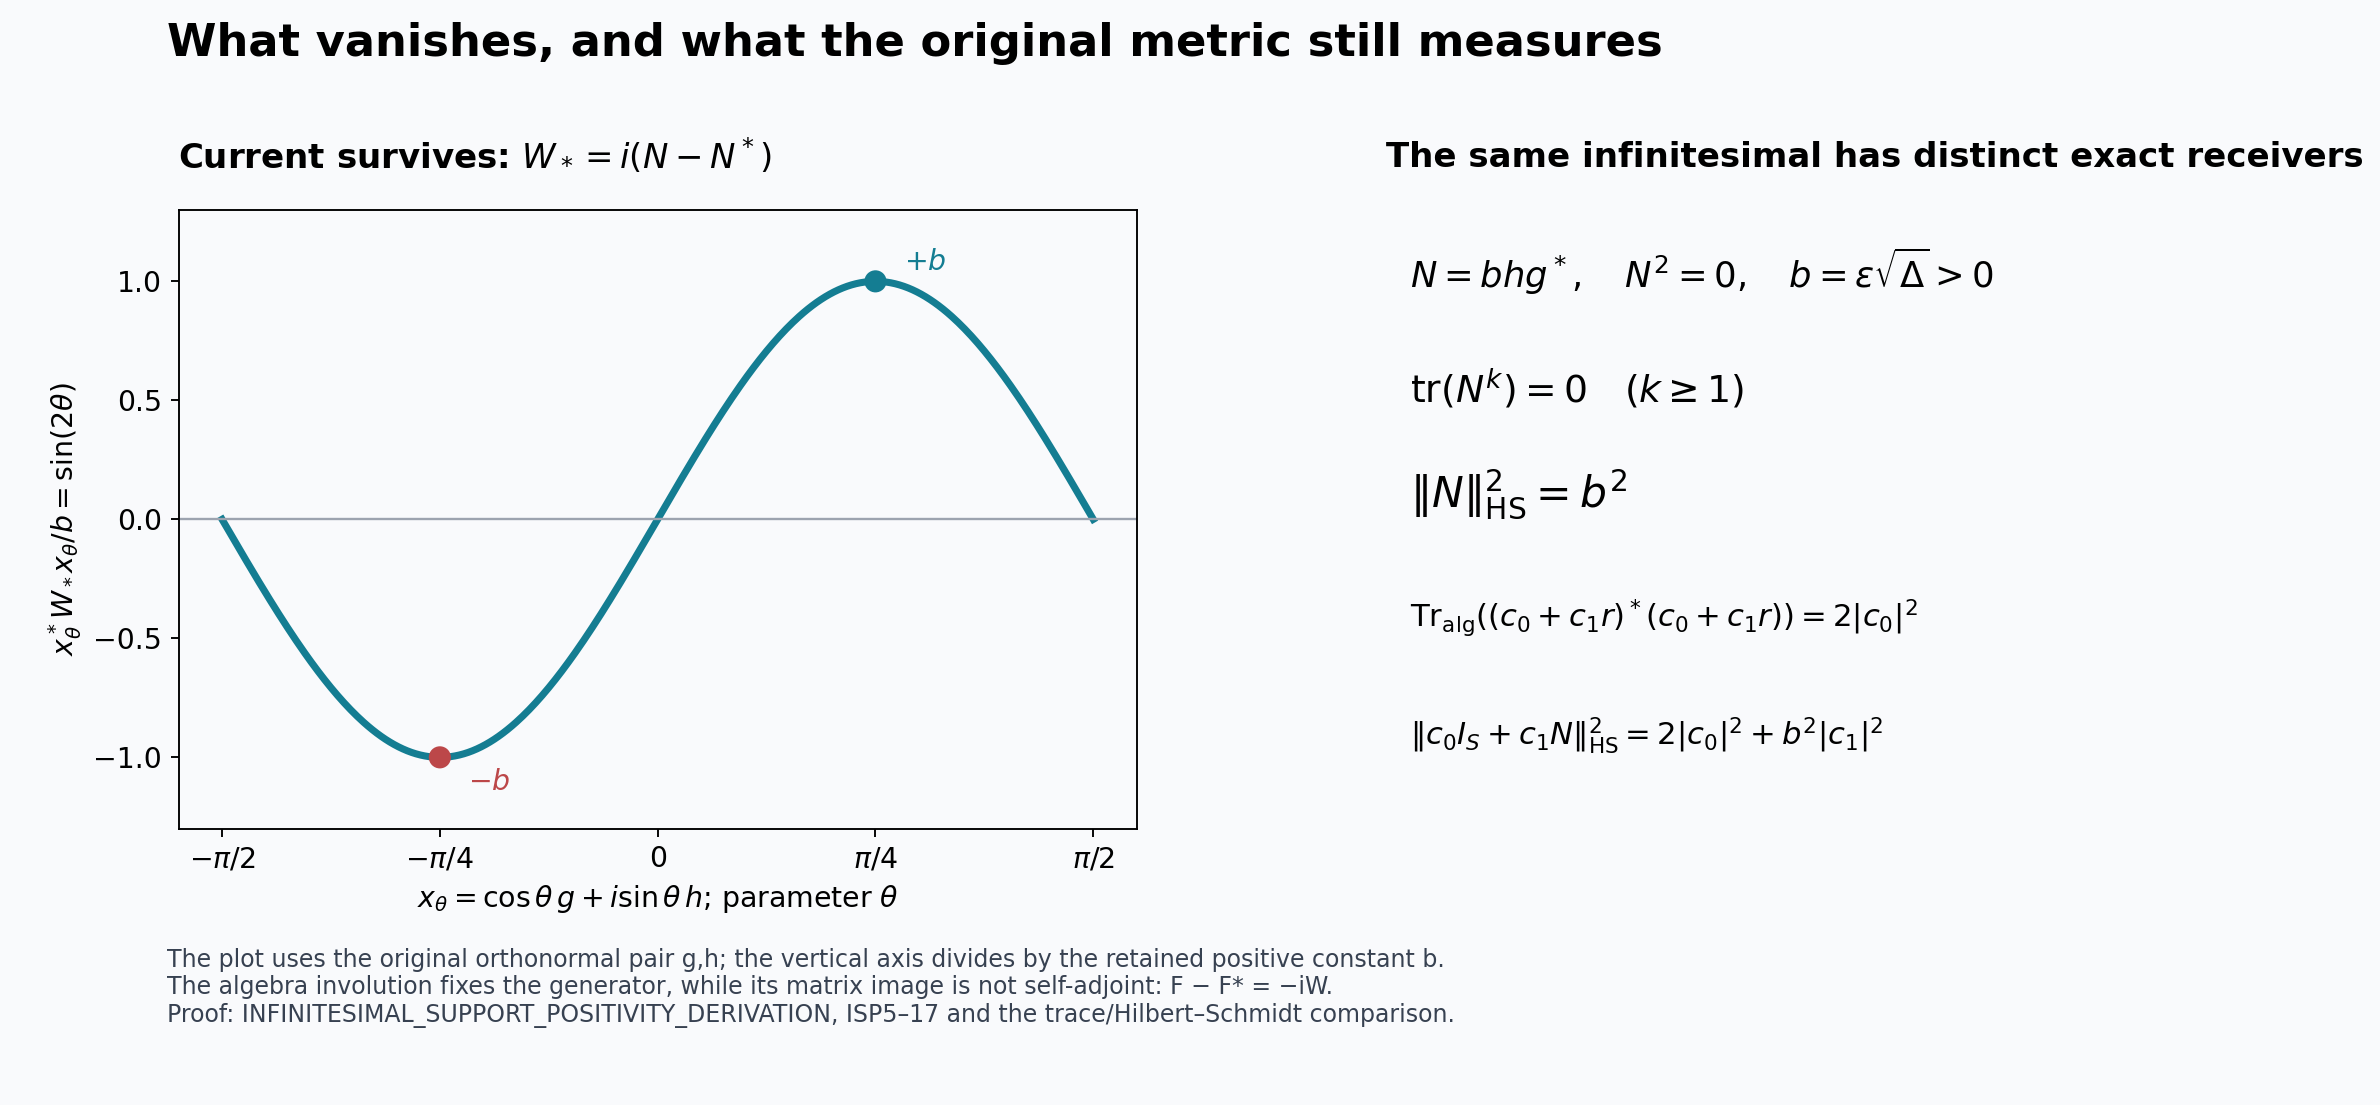
\includegraphics[keepaspectratio,alt={The same nonzero infinitesimal has zero algebraic trace and nonzero matrix norm; its current has both signs in the original metric. Proof: ISP5--ISP6, ISP18--ISP20, ISP45--ISP53.}]{figures/26_infinitesimal_forms.png}}
\caption{The same nonzero infinitesimal has zero algebraic trace and
nonzero matrix norm; its current has both signs in the original metric.
Proof: ISP5--ISP6, ISP18--ISP20, ISP45--ISP53.}
\end{figure}

\end{document}
